\documentclass[border=8pt]{standalone}
\usepackage{amsmath,amssymb}
\usepackage{tikz}
\usetikzlibrary{patterns}
\begin{document}
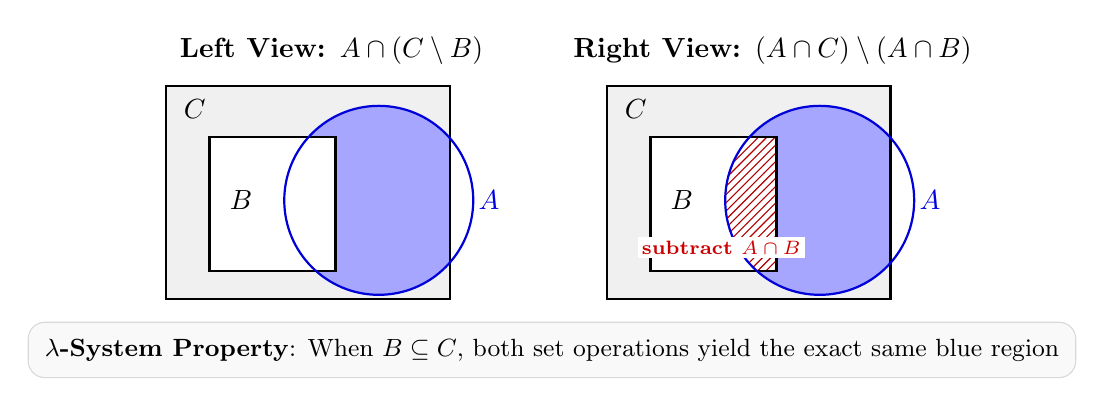
\begin{tikzpicture}[font=\small]
  % Left view: A \cap (C \setminus B)
  \begin{scope}[xshift=0cm]
    \node[font=\bfseries] at (2.1, 3.15) {Left View: $A \cap (C \setminus B)$};

    \draw[thick, fill=gray!12] (0, 0) rectangle (3.6, 2.7);
    \node[anchor=north west, font=\bfseries] at (0.1, 2.65) {$C$};

    \draw[thick, fill=white] (0.55, 0.35) rectangle (2.15, 2.05);
    \node[font=\bfseries] at (0.95, 1.25) {$B$};

    \begin{scope}
      \clip (2.7, 1.25) circle (1.2);
      \fill[blue!35] (0, 0) rectangle (3.6, 2.7);
      \fill[white] (0.55, 0.35) rectangle (2.15, 2.05);
    \end{scope}

    \draw[thick] (0, 0) rectangle (3.6, 2.7);
    \draw[thick] (0.55, 0.35) rectangle (2.15, 2.05);
    \draw[thick, draw=blue!85!black] (2.7, 1.25) circle (1.2);
    \node[font=\bfseries, text=blue!90!black] at (4.1, 1.25) {$A$};
  \end{scope}

  % Right view: (A \cap C) \setminus (A \cap B)
  \begin{scope}[xshift=5.6cm]
    \node[font=\bfseries] at (2.1, 3.15) {Right View: $(A \cap C) \setminus (A \cap B)$};

    \draw[thick, fill=gray!12] (0, 0) rectangle (3.6, 2.7);
    \node[anchor=north west, font=\bfseries] at (0.1, 2.65) {$C$};

    \draw[thick, fill=white] (0.55, 0.35) rectangle (2.15, 2.05);
    \node[font=\bfseries] at (0.95, 1.25) {$B$};

    \begin{scope}
      \clip (2.7, 1.25) circle (1.2);
      \fill[blue!35] (0, 0) rectangle (3.6, 2.7);
      \fill[white] (0.55, 0.35) rectangle (2.15, 2.05);
      \fill[pattern=north east lines, pattern color=red!70!black] (0.55, 0.35) rectangle (2.15, 2.05);
      \draw[thick, dashed, red!80!black] (0.55, 0.35) rectangle (2.15, 2.05);
    \end{scope}

    \draw[thick] (0, 0) rectangle (3.6, 2.7);
    \draw[thick] (0.55, 0.35) rectangle (2.15, 2.05);
    \draw[thick, draw=blue!85!black] (2.7, 1.25) circle (1.2);
    \node[font=\bfseries, text=blue!90!black] at (4.1, 1.25) {$A$};
    \node[font=\scriptsize\bfseries, text=red!80!black, fill=white, inner sep=1.5pt] at (1.45, 0.65) {subtract $A \cap B$};
  \end{scope}

  \node[align=center, fill=gray!5, draw=gray!30, rounded corners=6pt, inner sep=6pt] at (4.9, -0.65)
    {\textbf{$\lambda$-System Property}: When $B \subseteq C$, both set operations yield the exact same blue region};
\end{tikzpicture}
\end{document}
